\subsection{Footprint Refinements}\label{q:Footprint} 

The most impactful recommendation from Phase 1 was a substantial revision of the survey footprint. The recommended footprint, implemented in \texttt{baseline\_v2.0}, included a $\sim10\%$ area increase extending the WFD into low dust extinctions regions for extragalactic science and extended WFD-level coverage into high priority regions for Galactic science --- the Galactic Bulge and the Magellanic Clouds --- while removing high dust extinction Galactic Plane sky outside the Galactic Bulge from the WFD. A mini-survey area (a few 100's visits) was added to maintain some coverage of these parts of the sky. As a result of these changes, the overall area included in the survey was expanded and the number of visits per pointing dropped closer to the expected survey ``design'' values of 825 visits per pointing (see \citealt{LPM-17}) instead of the previous 900+ visits per pointing). See \citetalias{PSTN-053} Q1 \& 2 for details. 

The questions left open after the Phase 1 recommendations on the survey footprint were: 

\begin{enumerate}
\item What should the exact declination and/or dust extinction limits for the WFD region be? Should the Virgo cluster be added to the WFD?
\item What should the definition of the Galactic bulge region be? 
\item What fraction of time should be spent observing the Galactic Plane?
\item What fraction of time should be spent observing the NES?
\item What fraction of time should be spent covering the SCP?
\item What fraction of time should be spent on pencil beam surveys?
\end{enumerate}

\subsubsection{SCOC recommendations: executive summary}\label{rec:footprint_es}

 The SCOC reviewed all community-contributed reports and evaluated the impact of footprint changes on metrics contributed by the Survey Strategy team and by the community. The impact of footprint choices on many relevant metrics is shown in notebooks prepared by the Survey Strategy team.\footnote{Including \url{https://github.com/lsst-pst/survey_strategy/blob/main/fbs_2.0/SkyCoverage.ipynb} and \url{https://github.com/lsst-pst/survey_strategy/blob/main/fbs_2.0/Rolling\%20Cadence.ipynb}.}

{\bf The SCOC provides here a recommendation for the definition of the extragalactic footprint, NES, and SCP (see points 1, 4, and 5 below). The SCOC has finalized a recommendation on what fraction of time should be spent on the extragalactic \emph{vs} Galactic sky (point 3). Furthermore, there is general consensus that the current Galactic footprint definition is already a significant improvement over earlier definitions, but further enhancement can and should be considered keeping in mind that so long as the current overall extent and time spent on the Galactic sky is kept close to \texttt{baseline\_v2.0/2.1}, this will have no (negative) impact on the SCOC recommendations for the WFD and other areas of the sky. The SCOC continues to work towards a refinement of the Galactic footprint in collaboration with the Galactic science community}.\footnote{\label{fn:TVSSMWLVFoot}The most recent input into this process is the proposed Galactic Plane/Bulge coverage recommendation delivered by the TVS and SMWLV SCs, see \emph{Footprint exploration update: Update Galactic Science Mini-survey cadence/footprint} at \url{https://docs.google.com/presentation/d/1jjnTMeiwCLBhILF4lvgk8HzE3dkIwd9MCcWJR6a1B9A}.}
 
 Part of the effort of the refinement of the Galactic footprint is to assess whether higher cadence and/or a different filter balance in a subset of the Galactic Plane/Bulge area could lead to improved metrics for some Galactic science cases. However, the SCOC notes that, while a partial redistribution of a subset of the visits in the Bulge ``diamond''\footnote{See \url{https://community.lsst.org/t/july-2019-update/3760}.} to a broader area could be scientifically well motivated as it would cover a larger range of stellar populations and would distribute the potential for discovery over more diverse areas, a big part of the strength of Rubin’s LSST is its ability to cover large areas uniformly and deeply. Having a very tightly defined survey area that serves niche science cases would limit the diversity of science that can be done with the data in that part of the sky, and could thus reduce serendipitous discovery potential. Removing a large number of visits from the Bulge diamond would also result in less coverage of the part of the Galaxy that has the greatest density of stars and Galactic transients. \autoref{fig:fp} shows a comparison of the current (\texttt{baseline\_v2.X}) and recommended (\texttt{baseline\_v3.0}) 
 Galactic Plane footprint with the enhancement most recently proposed by the TVS and SMWLV SCs${fn:TVSSMWLVFoot}$.

\begin{figure}
    \centering
    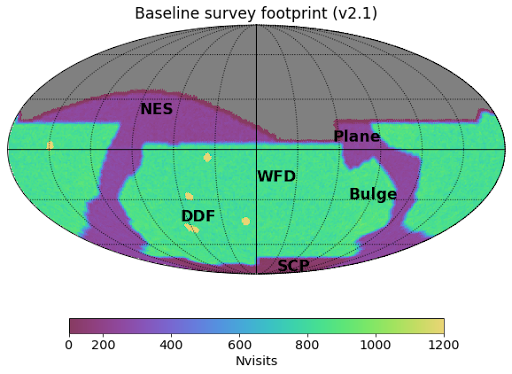
\includegraphics[width=0.5\textwidth]{figures/fp0.png}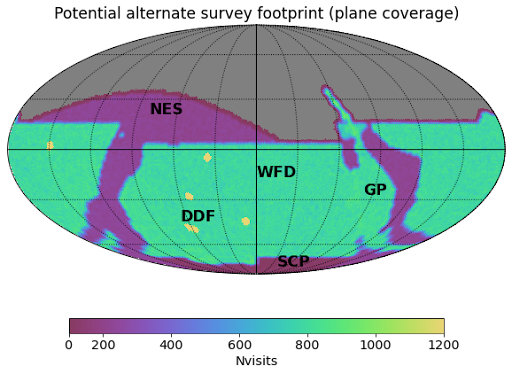
\includegraphics[width=0.5\textwidth]{figures/fp1.png}
    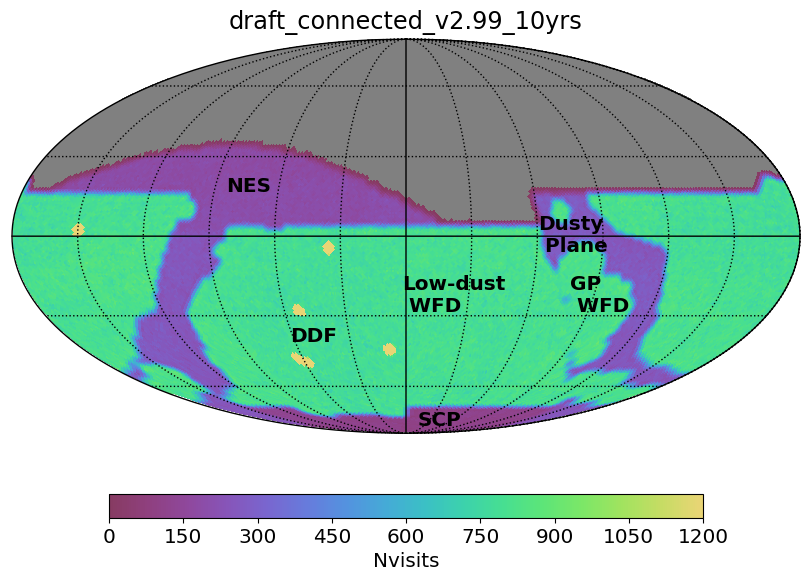
\includegraphics[width=0.5\textwidth]{figures/fp_299.png}
    \caption{Number of visits per field in three different \opsim\ simulations (colors saturated at 1,200 visits):  \texttt{baseline\_v2.1} (\emph{top left}); a simulation reproducing a TVS and SMWLV proposal for a prioritized Galactic Plane coverage${fn:TVSSMWLVFoot}$ 
    (\emph{top right}), and the footprint plan for the baseline simulation presented in this report (\emph{bottom}).}
    \label{fig:fp}
\end{figure}

\begin{figure}
    \centering
    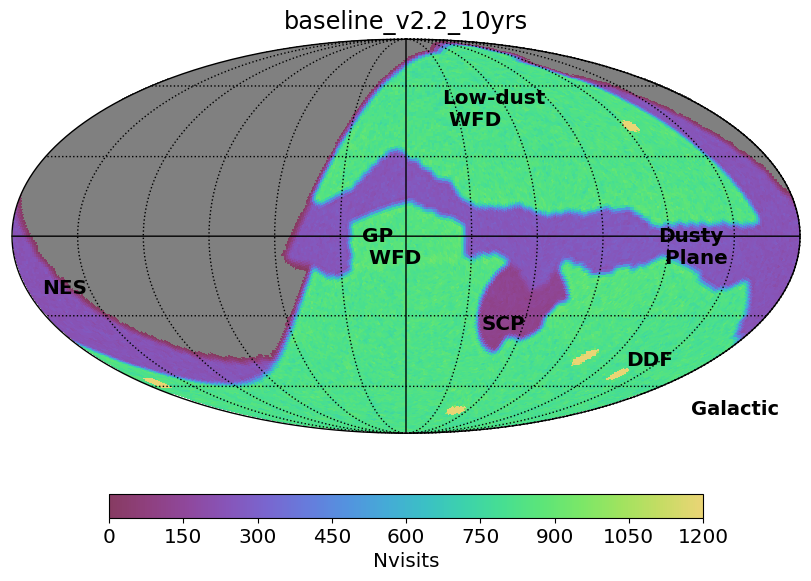
\includegraphics[width=0.5\textwidth]{figures/fp_200_gp.png}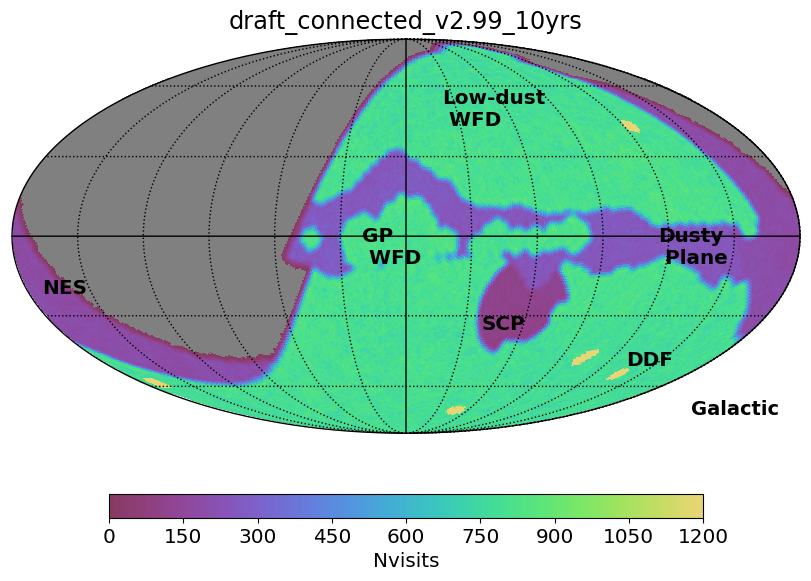
\includegraphics[width=0.5\textwidth]{figures/fp_299_gp.png}
    \caption{As \autoref{fig:fp} in a Galactic Plane projection for \texttt{baseline\_v2.2} (same footprint as \texttt{baseline\_v2.1}  \emph{left}) and for the current baseline (\emph{right}).}
    \label{fig:fp2}
\end{figure}

\subsubsection{SCOC recommendations: point by point answers}\label{rec:footprint}

\begin{enumerate}
\item 
The \texttt{baseline\_v2.X} WFD footprint appears to serve the scientific needs of the broad extragalactic community. The SCOC recommends that the \texttt{baseline\_v2.X} WFD low-dust footprint and overall time spent within it be preserved.

The current baseline implements an explicit WFD footprint request from DESC (which also benefits AGN, Galaxies, and extragalactic TVS science) to cover an extragalactic area of  $\sim18,0000~\degsq$ with $\ebv<0.2$~mag. To achieve this, \cite{2022ApJS..259...58L} recommended a footprint with $-70\degree<\mathrm{Dec}<+12.\degree5$
 over the portion of sky defined by the aforementioned extinction limit; an acceptable compromise, which avoids oversubscription of particular RA ranges and is adopted in the current baseline, is an upper limit of Dec~$<+15\degree$ for $\mathrm{RA}\sim7-18$~h and $\mathrm{Dec}<+3\degree$ for all other RA values.
 Synergies with other surveys (\emph{e.g.}, \emph{Euclid} and DESI) may motivate extending the survey declination limit even further into the northern sky, but there are currently no indicators that show strong benefits from this (metrics to measure the scientific advantages of overlap with these and other surveys while taking into account the expected image quality at high airmass should be developed to enable future reevaluations of the footprint northern limits). Nominal northern coverage of the Euclid region has been proposed as a microsurvey (\autoref{q:Micro}).

The SCOC recommends adding the Virgo Cluster to the WFD extragalactic region as part of the baseline survey (centered on RA$=186.75\degree$, Dec$=12.171$\degree, with a radius of $8.75\degree$).
Adding it represents a potentially important scientific payoff with negligible effects on the overall survey. Specifically, the addition of the Virgo Cluster in the WFD enables coverage of the highest stellar mass density in the nearby universe, with important benefits for local universe transient science and other key stellar populations such as globular clusters. Community support for this recommendation comes from the Galaxies SC (via their liaison).

\item As for the Galactic Bulge coverage and broader Galactic plane footprint, the SCOC is currently engaged in discussions with TVS and SMWLV representatives for further improvement (see above). \emph{ While no final recommendation is made for the Galactic plane footprint at this time, as described in \autoref{sec:shortrec} the distribution of observations within the Galactic footprint, including the filter balance and the different depth to which individual areas are covered, are compartmentalized decisions that can be optimized separately and do not significantly impact the rest of the survey.}

\item 
The SCOC recommends that the \texttt{baseline\_v3.0} simulation preserves the current \texttt{baseline\_2.X} total time allocation for the Galactic Plane. The amount of time spent observing the Plane as a whole in the current baseline represents the result of a compromise between competing scientific priorities and must be preserved in future strategies.  
%We did not find sufficient scientific support to justify taking a significant number of visits from the WFD, NES, or other minisurveys to allocate to the Plane. 
The distribution of visits within the Galactic Plane region and the Galactic Plane footprint are, however, a topic of active work and discussion (see point 2, as well as \autoref{q:Filters}, \autoref{q:Visits}, and \autoref{q:Rolling}).
%Therefore, additional time spent in the Plane should come primarily from other regions in the Plane/Bulge.


%However, it is possible that some additional time redistributed from the Bulge could be justified. We did not find sufficient scientific support to justify taking a significant number of visits from the WFD, NES or other minisurveys to allocate to the Plane: if the Plane is to have additional visits beyond the baseline, these should be reallocated from the Bulge.


\item The inclusion of the NES at the \texttt{baseline\_2.X} cadence level is supported by the SCOC. The SSSC metrics guide us in this recommendation.  A small reduction of NES coverage from the \texttt{baseline\_2.X} (from $\sim4.5$\% to $\sim3.5-4$\% of the survey time) is acceptable and it is implemented in \texttt{baseline\_v3.0}. Further changes at this level should be considered in a ``tweaking'' stage of the cadence in consultation with the SSSC. The current NES footprint extends from the northern boundary of the WFD and Galactic Plane up to $+ 10\degree$ ecliptic latitude; pushing this limit to lower ecliptic latitudes would lead to missing a substantial fraction of expected Solar System Objects (SSOs).

\item The SCOC recommends preserving the \texttt{baseline\_v2.0/2.1} time allocation for the SCP.
The main argument for the SCP is to allow for the opportunity to discover important Milky Way structures, such as dwarfs and streams, across the whole sky, making good use of Rubin as a survey instrument.  The current number of visits in the baseline is sufficient to have a significant scientific impact in this area, as can be seen from the Local Volume dwarfs metric and in the Local Volume notebook.\footnote{\url{https://github.com/lsst/rubin_sim_notebooks/blob/main/maf/science/Local_Volume_Dwarfs_Metric.ipynb}.} For example, compared to \citet{simon2019faintest}, LSST would probe new depths of dwarf discovery in the SCP, which is important for mapping the effect of the dark matter wake induced by the Large Magellanic Cloud \citep{garavito2021quantifying}. The exact filter distribution to be recommended for the SCP remains under investigation (see \autoref{q:Filters}).

\item 
To answer the question about the time to be spent on Galactic pencil-beam surveys, the SCOC needs more clarity on the definition of a pencil beam. Generally, we recommend balancing the benefits of segmentation of the Galactic Plane area into small subareas that serve niche science cases with the general benefits that LSST’s natural ability to cover large areas uniformly and deeply will afford. Outside of this balance being considered as part of the Galactic Plane/Bulge recommendation, pencil beams should perhaps be considered as micro- or nano-surveys (see \autoref{q:Micro}). Additionally, the use of alternative datasets (for example collected with DECam) that could complement LSST data and, if processed jointly, achieve specific science goals  should also be considered. \emph{At this stage the SCOC does not have a recommendation on the time to be spent on pencil-beam surveys of the Galactic Plane.}

\end{enumerate}

